% TODO: CRYPTO 2024's page limit is 30 pages excluding bibliography

\documentclass[runningheads]{llncs}
\usepackage[T1]{fontenc}
\usepackage{graphicx}
\usepackage{hyperref}
\usepackage{color}
\usepackage{amsmath,amsfonts}
\usepackage{algorithm}
\usepackage{algpseudocode}
\usepackage{caption}
\usepackage{multirow}
\usepackage{tikz}
\usetikzlibrary{positioning}

% Custom commands
\newcommand{\pke}{\texttt{PKE}}
\newcommand{\keygen}{\texttt{KeyGen}}
\newcommand{\encrypt}{\texttt{Enc}}
\newcommand{\decrypt}{\texttt{Dec}}
\newcommand{\kem}{\texttt{KEM}}
\newcommand{\encap}{\texttt{Encap}}
\newcommand{\decap}{\texttt{Decap}}
\newcommand{\etm}{\texttt{EtM}}  % encrypt-then-mac
\newcommand{\mac}{\texttt{MAC}}
\newcommand{\sign}{\texttt{Sign}}
\newcommand{\verify}{\texttt{Verify}}
\newcommand{\pk}{\texttt{pk}}
\newcommand{\sk}{\texttt{sk}}
\newcommand{\pco}{\texttt{PCO}}
\newcommand{\cvo}{\texttt{CVO}}
\newcommand{\leftsample}{\stackrel{\$}{\leftarrow}}
\newcommand{\llbrack}{[\![}
\newcommand{\rrbrack}{]\!]}
\newcommand{\norm}[1]{\left\lvert #1 \right\rvert}
\newcommand{\adv}{\texttt{Adv}}
\newcommand{\fotplus}{\texttt{FOT+}}
\newcommand{\us}{\mu s}
\newcommand{\wt}{\mathop{wt}}
\def\mlkemplus{\text{ML-KEM}^+}

\begin{document}
%
\title{Faster generic CCA secure KEM transformation using encrypt-then-MAC}
%
%\titlerunning{Abbreviated paper title}
% If the paper title is too long for the running head, you can set
% an abbreviated paper title here
%

\author{
    Ganyu Xu\inst{1} \and
    Guang Gong\inst{1} \and
    Kalikinkar Mandal\inst{2}
}
\authorrunning{G. Xu et al.}
% First names are abbreviated in the running head.
% If there are more than two authors, 'et al.' is used.
%

\institute{
    University of Waterloo, Waterloo, Ontario, Canada
    \email{\{g66xu,ggong\}@uwaterloo.ca} \and
    University of New Brunswick, Canada \email{kmandal@unb.ca}
}

\maketitle              % typeset the header of the contribution
%
\begin{abstract}
    Abstract needs to be rewritten because ML-KEM is not a suitable candidate. Instead, section 3 will be about the proof, section 4 will be a survey of existing public-key encryption schemes and a discussion of which ones are suitable, and section 5 will be about implementation and performance analysis with classic McEliece

\keywords{
    First keyword  \and Second keyword \and Another keyword.
}
\end{abstract}

\section{Introduction}\label{sec:introduction}
Introduction will need to be re-written. I will get back to it after writing section 2, 3, 4, 5

\section{Preliminaries}\label{sec:preliminaries}

\subsection{Public-key encryption scheme}
\paragraph{Syntax.} A public-key encryption scheme $\pke(\keygen, \encrypt, \decrypt)$ is a collection of three routines defined over some plaintext space $\mathcal{M}$ and some ciphertext space $\mathcal{C}$. Key generation $(\pk, \sk) \leftsample \keygen()$ is a randomized routine that returns a keypair. The encryption routine $\encrypt: (\pk, m) \mapsto c$ encrypts the input plaintext $m$ under the input public key $\pk$ and produces a ciphertext $c$. The decryption routine $\decrypt: (\sk, c) \mapsto m$ decrypts the input ciphertext $c$ under the input secret key $\sk$ and produces a plaintext $m$. Where the encryption routine is randomized, we denote the randomness by a coin $r \in \mathcal{R}$, where $\mathcal{R}$ is called the coin space. The decryption routine is assumed to always be deterministic.

\paragraph{Correctness.} Following the definition in \cite{DBLP:conf/eurocrypt/DworkNR04}, a $\pke$ is $\delta$-correct if:

\begin{equation*}
    E\left[\max_{m \in \mathcal{M}} P\left[\decrypt(\sk, c) \neq m \mid c \leftsample \encrypt(\pk, m)\right]\right] \leq \delta.
\end{equation*}

Where the expectation is taken with respect to the probability distribution of all possible keypairs $(\pk, \sk) \leftsample \texttt{PKE.KeyGen()}$. For many lattice-based cryptosystems, including ML-KEM, decryption failures could leak information about the secret key, although the probability of a decryption failure is low enough that classical adversaries cannot exploit decryption failure more than they can defeat the underlying lattice problem.

\paragraph{Rigidity.} %TODO: define rigidity, give citation

\paragraph{Security.} The security of public-key encryption is conventionally discussed within the context of adversarial games played between a challenger and an adversary \cite{DBLP:conf/stoc/GoldwasserM82}. There are two main types of games: i) in the one-wayness (OW-ATK) game, the adversary is given a random encryption, then asked to produce the correct decryption; ii) in the indistinguishability (IND-ATK) game, the adversary is given the encryption of one of two adversary-chosen plaintexts, then asked to decide which of the plaintexts corresponds with the given encryption. Depending on the attack model, the adversary may have access to various oracles. Within the context of public-key cryptography, adversaries are always assumed to have the public key with which they can mount chosen-plaintext attack (CPA). If the adversary has access to a plaintext-checking oracle (PCO) \cite{DBLP:conf/ctrsa/OkamotoP01} then it can mount plaintext-checking attack (PCA). Where the adversary has access to a decryption oracle, it can mount chosen-ciphertext attacks (CCA). 

\begin{figure}[h]
    \centering

    \begin{minipage}[t]{0.4\textwidth}
        \begin{algorithm}[H]
            \caption*{\texttt{OW-ATK} Game}
            \begin{algorithmic}[1]
                \State $(\pk, \sk) \leftsample \keygen(1^\lambda)$
                \State $m^\ast \leftsample \mathcal{M}$
                \State $c^\ast \leftsample \encrypt(\pk, m^\ast)$
                \State $\hat{m} \leftsample A^{\mathcal{O}_\texttt{ATK}}(1^\lambda, \pk, c^\ast)$
                \State \Return $\llbrack \hat{m} = m^\ast \rrbrack$
            \end{algorithmic}
        \end{algorithm}
    \end{minipage}
    % \hfill
    \begin{minipage}[t]{0.4\textwidth}
        \begin{algorithm}[H]
            \caption*{\texttt{IND-ATK} Game}
            \begin{algorithmic}[1]
                \State $(\pk, \sk) \leftsample \keygen(1^\lambda)$
                \State $(m_0, m_1) \leftsample A^{\mathcal{O}_\texttt{ATK}}(1^\lambda, \pk)$
                \State $b \leftsample \{0,1\}$
                \State $c^\ast \leftsample \encrypt(\pk, m_b)$
                \State $\hat{b} \leftsample A^{\mathcal{O}_\texttt{ATK}}(1^\lambda, \pk, c^\ast)$
                \State \Return $\llbrack \hat{b} = b \rrbrack$
            \end{algorithmic}
        \end{algorithm}
    \end{minipage}
    % \begin{minipage}[t]{0.33\textwidth}
    %     \begin{algorithm}[H]
    %         \caption*{$\mathcal{O}_\pco(m, c)$}
    %         \begin{algorithmic}[1]
    %             \State \Return $\llbrack m = \decrypt(\sk, c) \rrbrack$
    %         \end{algorithmic}
    %     \end{algorithm}
    %     \begin{algorithm}[H]
    %         \caption*{$\mathcal{O}_\decrypt(c)$}
    %         \begin{algorithmic}[1]
    %             \State \Return $\decrypt(\sk, c)$
    %         \end{algorithmic}
    %     \end{algorithm}
    % \end{minipage}
    \caption{The one-way game, indistinguishability game, plaintext-checking oracle (PCO), and decryption oracle. $\texttt{ATK} \in \{\texttt{CPA}, \texttt{PCA}, \texttt{CCA}\}$}
\end{figure}

The advantage of an adversary in the \texttt{OW-ATK} game is the probability that it outputs the correct decryption. The advantage of an adversary in the \texttt{IND-ATK} game is defined below. A PKE is \texttt{OW-ATK}/\texttt{IND-ATK} secure if no efficient adversary has non-negligible advantage in the corresponding security game.

\begin{equation*}
    \texttt{Adv}_\texttt{IND-ATK}(A) = \left\vert P\left[A^{\mathcal{O}_\texttt{ATK}}(1^\lambda, \pk, c^\ast) = b \right] - \frac{1}{2} \right\vert.
\end{equation*}

\subsection{Key encapsulation mechanism (KEM)}
\paragraph{Syntax.} A key encapsulation mechanism $\kem(\keygen, \encap, \decap)$ is a collection of three routines defined over some ciphertext space $\mathcal{C}$ and some key space $\mathcal{K}$. The key generation routine takes the security parameter $1^\lambda$ and outputs a keypair $(\pk, \sk) \leftsample \keygen(1^\lambda)$. $\encap(\pk)$ is a probabilistic routine that takes a public key $\pk$ and outputs a pair of values $(c, K)$ where $c \in \mathcal{C}$ is the ciphertext (also called encapsulation) and $K \in \mathcal{K}$ is the shared secret (also called session key). $\decap(\sk, c)$ is a deterministic routine that takes the secret key $\sk$ and the encapsulation $c$ and returns the shared secret $K$ if the ciphertext is valid. Some KEM constructions use explicit rejection, where if $c$ is invalid then $\decap$ will return a rejection symbol $\bot$; other KEM constructions use implicit rejection, where if $c$ is invalid then $\decap$ will return a fake session key that depends on the ciphertext and some other secret values.

\paragraph{Security.} The security of a KEM is similarly discussed in adversarial games (Figure \ref{fig:kem-game}), although the win conditions differ slightly from the win conditions of a PKE indistinguishability game. In a KEM's indistinguishability game, an adversary is given the public key and a challenge ciphertext, then asked to distinguish a pseudorandom shared secret $K_0$ associated with the challenge ciphertext from a truly random bit string of equal length.

\begin{figure}[H]
    \centering
    \begin{minipage}[t]{0.49\textwidth}
        \begin{algorithm}[H]
            \caption*{\texttt{IND-ATK} game}
            \begin{algorithmic}[1]
                \State $(\pk, \sk) \leftsample \keygen(1^\lambda)$
                \State $(c^\ast, K_0) \leftsample \encap(\pk)$
                \State $K_1 \leftsample \mathcal{K}$
                \State $b \leftsample \{0, 1\}$
                \State $\hat{b} \leftsample A^{\mathcal{O}_\texttt{ATK}}(
                    1^\lambda, \pk, c^\ast, K_b
                )$
                \State \Return $\llbrack \hat{b} = b \rrbrack$
            \end{algorithmic}
        \end{algorithm}
    \end{minipage}\hfill
    \begin{minipage}[t]{0.49\textwidth}
        \begin{algorithm}[H]
        \caption*{$\mathcal{O}_\decap(c)$}
        \begin{algorithmic}[1]
            \State \Return $\decap(\sk, c)$
        \end{algorithmic}
        \end{algorithm}
    \end{minipage}
    \caption{\texttt{IND-ATK} game for KEM and decapsulation oracle $\mathcal{O}_\decap$}\label{fig:kem-game}
\end{figure}

The decapsulation oracle $\mathcal{O}^\decap$ takes a ciphertext $c$ and returns the output of the $\decap$ routine using the secret key. The advantage of an IND-CCA adversary $\mathcal{A}_\texttt{IND-CCA}$ is defined by the adversary's ability to correctly distinguish the two cases beyond a blind guess:

\begin{equation*}
    \adv_\texttt{IND-CCA}(A) = \norm{
        P[A^{\mathcal{O}_\decap}(a^\lambda, \pk, c^\ast, K_b) = b] - \frac{1}{2}
    }.
\end{equation*}

A KEM is \texttt{IND-ATK} secure if no efficient adversary has non-negligible advantage in the corresponding security game.

\subsection{Message authentication code (MAC)}\label{sec:message-authentication-code}
\paragraph{Syntax.} A message authentication code $\mac(\keygen, \sign, \verify)$ is a collection of routines defined over some key space $\mathcal{K}$, some message space $\mathcal{M}$, and some tag space $\mathcal{T}$. The signing routine $\sign(k, m)$ authenticates the message $m$ under the secret key $k$ by producing a tag $t$ (also called digest) (we define the process that generates an authentication tag $t$ over message $m$ a \textit{signing routine} in this paper). The verification routine $\verify(k, m, t)$ takes the triplet of secret key $k$, message $m$, and tag $t$, and outputs $\texttt{1}$ if the message-tag pair is valid under the secret key, or $\texttt{0}$ otherwise. Many MAC constructions are deterministic. For these constructions it is simpler to denote the signing routine by $t \leftarrow \mac(k, m)$ and perform verification using a simple comparison.

\paragraph{Security.} The security of a MAC is defined in an adversarial game in which an adversary, with access to a MAC oracle that can answer signing queries $\mac(k, m) \leftarrow \mathcal{O}_\mac(m)$, tries to forge a new valid message-tag pair that has never been queried before. The ability to access a MAC oracle is called \emph{chosen-message attack (CMA)}. The ability to produce a valid tag on some arbitrary message is called \emph{existential forgery}. The existential unforgeability under chosen message attack (EUF-CMA) game is shown below:

\begin{figure}[H]
    \centering
    \begin{minipage}[t]{0.53\textwidth}
        \begin{algorithm}[H]
            \caption*{\texttt{EUF-CMA} game}
            \begin{algorithmic}[1]
                \State $k^\ast \leftsample \mathcal{K}$
                \State $(\hat{m}, \hat{t}) \leftsample \mathcal{A}^{\mathcal{O}_\mac}()$
                \State \Return $
                    \llbrack \verify(k^\ast, \hat{m}, \hat{t}) 
                    \land (\hat{m}, \hat{t}) \not\in \mathcal{O}_\mac
                    \rrbrack
                $
            \end{algorithmic}
        \end{algorithm}
    \end{minipage}\hspace{0.3cm}
    \begin{minipage}[t]{0.4\textwidth}
        \begin{algorithm}[H]
            \caption*{MAC oracle $\mathcal{O}_\mac(m)$}
            \begin{algorithmic}[1]
                \State \Return $\mac(k^\ast, m)$
            \end{algorithmic}
        \end{algorithm}
    \end{minipage}
    \caption{The existential forgery game and the MAC oracle}\label{fig:euf-cma-game}
\end{figure}

The advantage $\adv_\texttt{EUF-CMA}$ of the existential forgery adversary is the probability that it wins the EUF-CMA game. Some MACs are one-time existentially unforgeable, meaning that each secret key can be used to authenticate only a single message. The corresponding security game is modified such that the MAC oracle will only answer a single signing query.

% \section{Encrypt-then-MAC: new generic IND-CCA KEM transformation}\label{sec:the-encrypt-then-mac-transformation}
\section{The encrypt-then-MAC transformation}\label{sec:the-encrypt-then-mac-transformation}
\paragraph{Our technique.} We introduce our encrypt-then-MAC transformation that transforms a OW-PCA secure PKE and an one-time existentially unforgeable MAC into an IND-CCA secure KEM. Our scheme mainly differs from DHIES in its versatility and input requirement. Whereas the IND-CCA security of DHIES reduces specifically to the Gap Diffie-Hellman assumption, the chosen-ciphertext security of the encrypt-then-MAC KEM reduces more generally to the OW-PCA security \cite{DBLP:conf/ctrsa/OkamotoP01} of the input scheme. In addition, we propose that because each call to encapsulation samples a fresh PKE plaintext, the encrypt-then-MAC KEM can be instantiated with one-time secure MAC such as Poly1305 for further performance improvements (Abdalla, Rogaway, and Bellare originally proposed to use HMAC and CBC-MAC, which are many-time secure MAC but less efficient than one-time MAC, see Section \ref{sec:choosing-a-message-authenticator}). The encapsulation data flow is illustrated in Figure \ref{fig:etm-diagram}.

\begin{figure}[H]
    \centering
    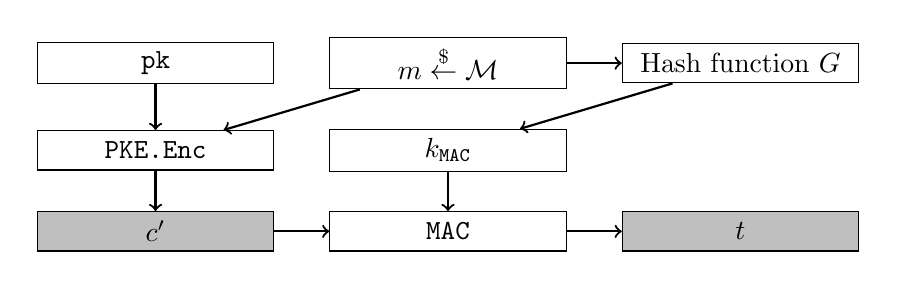
\begin{tikzpicture}
        \tikzstyle{rect} = [draw, rectangle, minimum width=3cm, minimum height=0.5cm]
        \tikzstyle{filledrect} = [draw, rectangle, minimum width=3cm, minimum height=0.5cm, fill=lightgray]
        \matrix [column sep=7mm, row sep=5mm] {
            \node (pk) [rect] {$\pk$}; &
            \node (m) [rect] {$m \leftsample \mathcal{M}$}; &
            \node (hashg) [rect] {Hash function $G$}; \\
            \node (pkeenc) [rect] {$\texttt{PKE.Enc}$}; &
            \node (mackey) [rect] {$k_\mac$}; \\
            \node (ct) [filledrect] {$c^\prime$}; &
            \node (mac) [rect] {$\mac$}; &
            \node (tag) [filledrect] {$t$}; \\
        };
        \draw[->, thick] (pk) -- (pkeenc);
        \draw[->, thick] (m) -- (pkeenc);
        \draw[->, thick] (m) -- (hashg);
        \draw[->, thick] (hashg) -- (mackey);
        \draw[->, thick] (pkeenc) -- (ct);
        \draw[->, thick] (mackey) -- (mac);
        \draw[->, thick] (ct) -- (mac);
        \draw[->, thick] (mac) -- (tag);
    \end{tikzpicture}

    \caption{Combining PKE with MAC using encrypt-then-MAC to ensure ciphertext integrity}\label{fig:etm-diagram}
\end{figure}

In Section \ref{sec:proof-of-theorem} we reduce the IND-CCA security of the KEM tightly to the OW-PCA security of the underlying PKE, and non-tightly to the unforgeability of the MAC. In Section \ref{sec:elgamal-is-ow-pca}, we show that DHIES is a special case of the encrypt-then-MAC transformation by reducing the OW-PCA security of the ElGamal cryptosystem to the Gap Diffie-Hellman assumption.

\subsection{The generic KEM construction}
Let $\mathcal{B}^\ast$ denote the set of finite bit strings. Let $\pke(\keygen, \encrypt, \decrypt)$ be a public-key encryption scheme defined over message space $\mathcal{M}$ and ciphertext space $\mathcal{C}$. Let $\mac: \mathcal{K}_\mac \times \mathcal{B}^\ast \rightarrow \mathcal{T}$ be a deterministic message authentication code that takes a key $k \in \mathcal{K}_\mac$, some message $m \in \mathcal{B}^\ast$, and outputs a tag $t \in \mathcal{T}$. Let $G: \mathcal{M} \rightarrow \mathcal{K}_\mac$ be a hash function that maps from $\pke$'s plaintext space to $\mac$'s key space. Let $H: \mathcal{B}^\ast \rightarrow \mathcal{K}_\kem$ be a hash function that maps bit strings into the set of possible shared secrets. The encrypt-then-MAC transformation $\etm[\pke, \mac, G, H]$ constructs a key encapsulation mechanism $\kem_\etm(\keygen, \encap, \decap)$, whose routines are described in Figure \ref{fig:etm-routines}.

\begin{figure}[H]
    \centering
    \begin{minipage}[t]{0.5\textwidth}
        \begin{algorithm}[H]
            \caption*{$\kem_\etm.\keygen()$}
            \begin{algorithmic}[1]
                \State $(\pk, \sk^\prime) \leftsample \pke\texttt{.}\keygen()$
                \State $z \leftsample \mathcal{M}$
                \State $\sk \leftarrow (\sk^\prime, z)$
                \State \Return $(\pk, \sk)$
            \end{algorithmic}
        \end{algorithm}
        \begin{algorithm}[H]
            \caption*{$\kem_\etm.\encap(\pk)$}
            \begin{algorithmic}[1]
                \State $m \leftsample \mathcal{M}$
                \State $k \leftarrow G(m)$
                \State $c^\prime \leftsample \pke\texttt{.}\encrypt(\pk, m)$
                \State $t \leftarrow \mac(k, c^\prime)$
                \State $c \leftarrow (c^\prime, t)$
                \State $K \leftarrow H(m, c)$
                \State \Return $(c, K)$
            \end{algorithmic}
        \end{algorithm}
    \end{minipage}\hfill
    \begin{minipage}[t]{0.49\textwidth}
        \begin{algorithm}[H]
            \caption*{$\kem_\etm.\decap(\sk, c)$}
            \begin{algorithmic}[1]
                \State $(c^\prime, t) \leftarrow c$
                \State $(\sk^\prime, z) \leftarrow \sk$
                \State $\hat{m} \leftarrow \pke\texttt{.}\decrypt(\sk^\prime, c^\prime)$
                \State $\hat{k} \leftarrow G(\hat{m})$
                \If{$\mac(\hat{k}, c^\prime) = t$}
                    \State $K \leftarrow H(\hat{m}, c)$
                \Else
                    % This is directly copied from ML-KEM, DO NOT CHANGE
                    \State $K \leftarrow H(z, c)$
                \EndIf
                \State \Return $K$
            \end{algorithmic}
        \end{algorithm}
    \end{minipage}
    \caption{The encrypt-then-MAC transformation builds a KEM, denoted by $\kem_\etm$, using a $\pke(\keygen, \encrypt, \decrypt)$, a $\mac$, and two hash functions $G, H$}\label{fig:etm-routines} 
\end{figure}

% The key generation routine of $\kem_\etm$ is largely identical to that of the $\pke$, only a secret value $z$ is sampled as the implicit rejection symbol. In the encapsulation routine, a MAC key is derived from the randomly sampled plaintext, then used to sign the unauthenticated ciphertext $c^\prime$. Finally, the unauthenticated ciphertext $c^\prime$ and the tag $t$ combine into the authenticated ciphertext $c$ that would be transmitted to the peer. In the decapsulation routine, the decryption $\hat{m}$ of the unauthenticated ciphertext is used to re-derive the MAC key $\hat{k}$, which is then used to re-compute the tag $\hat{t}$. The ciphertext is considered valid if and only if the recomputed tag is identical to the input tag.

Since the encrypt-then-MAC transformation removes re-encryption in decapsulation, there is no longer the need for fixing the pseudorandom coin $r$ in the PKE's encryption routine. If the input PKE is already rigid, then the shared secret may be derived from hashing the PKE plaintext alone. However, if the input PKE is not rigid, then the shared secret must be derived from hashing both the PKE plaintext and the PKE ciphertext. 

\paragraph{Security analysis.} The CCA security of the encrypt-then-MAC scheme can be intuitively argued through an adversary's inability to learn additional information from the decapsulation oracle. For an adversary $A$ to produce a valid tag $t$ for some unauthenticated ciphertext $c^\prime$ under the symmetric key $k \leftarrow G(\decrypt(\sk^\prime, c^\prime))$ implies that $A$ must either know the symmetric key $k$ or produce a forgery. Under the random oracle model, $A$ also cannot know $k$ without knowing its pre-image $\decrypt(\sk^\prime, c^\prime)$, so $A$ must either have produced $c^\prime$ honestly, or have broken the one-way security of $\pke$. This means that the decapsulation oracle will not give out information on decryption that the adversary does not already know. 

However, a decapsulation oracle can still give out some information: for a known plaintext $m$, all possible encryptions $c^\prime \leftsample \encrypt(\pk, m)$ can be correctly signed, while ciphertexts that don't decrypt back to $m$ cannot be correctly signed. This means that a decapsulation oracle can be converted into a plaintext-checking oracle, so every chosen-ciphertext attack against the KEM can be converted into a plaintext-checking attack against the underlying PKE.

On the other hand, if the underlying PKE is OW-PCA secure and the underlying MAC is one-time existentially unforgeable, then the encrypt-then-MAC KEM is IND-CCA secure:

\begin{theorem}\label{thm:ow-pca-implies-kem-ind-cca2}
    For every \texttt{IND-CCA} adversary $A$ against $\kem_\etm$ that makes $q$ decapsulation queries, there exists an \texttt{OW-PCA} adversary $B$ who makes at least $q$ plaintext-checking queries against the underlying $\pke$, and an one-time existential forgery adversary $C$ against the underlying $\mac$ such that

    \begin{equation*}
        \texttt{Adv}_\texttt{IND-CCA}(A) \leq q \cdot \adv_\texttt{OT-MAC}(C) + 2 \cdot \texttt{Adv}_\texttt{OW-PCA}(B).
    \end{equation*}
\end{theorem}

\subsection{Proof of Theorem \ref{thm:ow-pca-implies-kem-ind-cca2}}\label{sec:proof-of-theorem}
We will prove Theorem \ref{thm:ow-pca-implies-kem-ind-cca2} using a sequence of game. A summary of the the sequence of games can be found in Figure \ref{fig:etm-ind-cc2-sequence-of-games} and \ref{fig:ow-pca-simulates-game-3}. From a high level we made three incremental modifications to the IND-CCA game for $\kem_\etm$: \begin{enumerate}
    \setlength\itemsep{0.1em}
    \item Replace the true decapsulation oracle with a simulated decapsulation oracle
    \item Replace the pseudorandom MAC key $k^\ast \leftarrow G(m^\ast)$ with a truly random $k^\ast \leftsample \mathcal{K}_\mac$
    \item Replace the pseudorandom shared secret $K_0 \leftarrow H(m^\ast, c)$ with a truly random shared secret $K_0 \leftsample \mathcal{K}_\kem$
\end{enumerate}

A OW-PCA adversary can then simulate the modified IND-CCA game for the KEM adversary, and the advantage of the OW-PCA adversary is associated with the probability of certain behaviors of the KEM adversary.

\begin{figure}[H]
    \centering
    \begin{minipage}[t]{0.5\textwidth}
        \begin{algorithm}[H]
            \caption*{\texttt{IND-CCA} game for $\kem_\etm$}
            \begin{algorithmic}[1]
                \State $(\pk, \sk) \leftsample \kem_\etm\texttt{.}\keygen()$
                \State $m^\ast \leftsample \mathcal{M}$
                \State $c^\prime \leftsample \pke\texttt{.}\encrypt(\pk, m^\ast)$
                \State $k^\ast \leftarrow G(m^\ast)$
                    \Comment{Game 0-1}
                \State $k^\ast \leftsample \mathcal{K}_\mac$
                    \Comment{Game 2-3}
                \State $t \leftarrow \mac(k^\ast, c^\prime)$
                \State $c^\ast \leftarrow (c^\prime, t)$
                \State $K_0 \leftarrow H(m^\ast, c^\ast)$
                    \Comment{Game 0-2}
                \State $K_0 \leftsample \mathcal{K}_\kem$
                    \Comment{Game 3}
                \State $K_1 \leftsample \mathcal{K}_\kem$
                \State $b \leftsample \{0,1\}$
                \State $\hat{b} \leftarrow A^{\mathcal{O}^\decap}(\pk, c^\ast, K_b)$
                    \Comment{Game 0}
                \State $\hat{b} \leftarrow A^{\mathcal{O}^\decap_1}(\pk, c^\ast, K_b)$
                    \Comment{Game 1-3}
                \State \Return $\llbrack \hat{b} = b \rrbrack$
            \end{algorithmic}
        \end{algorithm}
        \begin{algorithm}[H]
            \caption*{Hash oracle $\mathcal{O}^G(m)$}
            \begin{algorithmic}[1]
                \If{$\exists (\tilde{m}, \tilde{k}) \in \mathcal{L}^G : \tilde{m} = m$}
                    \State \Return $\tilde{k}$
                \EndIf
                \State $k \leftsample \mathcal{K}_\mac$
                \State $\mathcal{L}^G \leftarrow \mathcal{L}^G \cup \{(m, k)\}$
                \State \Return $k$
            \end{algorithmic}
        \end{algorithm}
    \end{minipage}
    \begin{minipage}[t]{0.49\textwidth}
        \begin{algorithm}[H]
            \caption*{Decap oracle $\mathcal{O}^\decap(c)$}
            \begin{algorithmic}[1]
                \State $(c^\prime, t) \leftarrow c$
                \State $\hat{m} = \decrypt(\sk^\prime, c^\prime)$
                \State $\hat{k} \leftarrow G(\hat{m})$
                \If{$\mac(\hat{k}, c^\prime) = t$}
                    \State $K \leftarrow H(\hat{m}, c)$
                \Else 
                    \State $K \leftarrow H(z, c)$
                \EndIf 
                \State \Return $K$
            \end{algorithmic}
        \end{algorithm}
        \vspace{-0.5cm}
        \begin{algorithm}[H]
            \caption*{$\mathcal{O}^\decap_1(c)$}
            \begin{algorithmic}[1]
                \State $(c^\prime, t) \leftarrow c$
                \If{$\exists (\tilde{m}, \tilde{k}) \in \mathcal{L}^G : 
                    \tilde{m} = \decrypt(\sk^\prime, c^\prime)
                    \land \mac(\tilde{k}, c^\prime) = t
                $}
                    \State $K \leftarrow H(\tilde{m}, c)$
                \Else
                    \State $K \leftarrow H(z, c)$
                \EndIf
                \State \Return $K$
            \end{algorithmic}
        \end{algorithm}
        \vspace{-0.5cm}
        \begin{algorithm}[H]
            \caption*{$\mathcal{O}^H(m, c)$}
            \begin{algorithmic}[1]
                \If{$\exists (\tilde{m}, \tilde{c}, \tilde{K}) \in \mathcal{L}^H : \tilde{m} = m \land \tilde{c} = c$}
                    \State \Return $\tilde{K}$
                \EndIf
                \State $K \leftsample \mathcal{K}_\kem$
                \State $\mathcal{L}^H \leftarrow \mathcal{L}^H \cup \{(m, c, K)\}$
                \State \Return $K$
            \end{algorithmic}
        \end{algorithm}
    \end{minipage}
    \caption{Sequence of games in the proof of Theorem \ref{thm:ow-pca-implies-kem-ind-cca2}}\label{fig:etm-ind-cc2-sequence-of-games}
\end{figure}
\begin{figure}[H]
    \begin{minipage}[t]{0.49\textwidth}
        \begin{algorithm}[H]
            \caption*{$B(\pk, {c^\prime}^\ast)$}
            \begin{algorithmic}[1]
                \State $z \leftsample \mathcal{M}$
                \State $k \leftsample \mathcal{K}_\mac$
                \State $t \leftarrow \mac(k, {c^\prime}^\ast)$
                \State $c^\ast \leftarrow ({c^\prime}^\ast, t)$
                \State $K \leftsample \mathcal{K}_\kem$
                \State $\hat{b} \leftarrow A^{
                    \mathcal{O}^\decap_B, \mathcal{O}^G_B, \mathcal{O}^H_B
                }(\pk, c^\ast, K)$
                \If{$\texttt{ABORT}(m)$}
                    \State \Return $m$
                \EndIf
            \end{algorithmic}
        \end{algorithm}\vspace{-0.5cm}
        \begin{algorithm}[H]
            \caption*{$\mathcal{O}^H_B(m, c)$}
            \begin{algorithmic}
                \If{$\pco(m, {c^\prime}^\ast) = 1$}
                    \State $\texttt{ABORT}(m)$
                \EndIf
                \If{$
                    \exists (\tilde{m}, \tilde{c}, \tilde{K}) \in \mathcal{L}^H 
                    : \tilde{m} = m \land \tilde{c} = c
                $}
                    \State \Return $\tilde{K}$
                \EndIf
                \State $K \leftsample \mathcal{K}_\kem$
                \State $\mathcal{L}^H \leftarrow \mathcal{L}^H \cup \{(m, c, K)\}$
                \State \Return $K$
            \end{algorithmic}
        \end{algorithm}
    \end{minipage}\hfill
    \begin{minipage}[t]{0.49\textwidth}
        \begin{algorithm}[H]
            \caption*{$\mathcal{O}^\decap_B(c)$}
            \begin{algorithmic}[1]
                \State $(c^\prime, t) \leftarrow c$
                \If{$\exists (\tilde{m}, \tilde{k}) \in \mathcal{L}^G : 
                    % \tilde{m} = \decrypt(\sk^\prime, c^\prime)
                    \pco(\tilde{m}, c^\prime) = 1
                    \land \mac(\tilde{k}, c^\prime) = t
                $}
                    \State $K \leftarrow H(\tilde{m}, c)$
                \Else
                    \State $K \leftarrow H(z, c)$
                \EndIf
                \State \Return $K$
            \end{algorithmic}
        \end{algorithm}
        \begin{algorithm}[H]
            \caption*{$\mathcal{O}^G_B(m)$}
            \begin{algorithmic}[1]
                \If{$\pco(m, {c^\prime}^\ast) = 1$}
                    \State $\texttt{ABORT}(m)$
                \EndIf
                \If{$\exists (\tilde{m}, \tilde{k}) \in \mathcal{L}^G : \tilde{m} = m$}
                    \State \Return $\tilde{k}$
                \EndIf
                \State $k \leftsample \mathcal{K}_\mac$
                \State $\mathcal{L}^G \leftarrow \mathcal{L}^G \cup \{(m, k)\}$
                \State \Return $k$
            \end{algorithmic}
        \end{algorithm}
    \end{minipage}
    \caption{OW-PCA adversary $B$ simulates game 3 for IND-CCA adversary $A$ in the proof for Theorem \ref{thm:ow-pca-implies-kem-ind-cca2}}\label{fig:ow-pca-simulates-game-3}
\end{figure}


\begin{proof}
    \emph{Game 0} is the standard KEM IND-CCA game. The decapsulation oracle $\mathcal{O}^\decap$ executes the decapsulation routine using the challenge keypair and return the results faithfully. The queries made to the hash oracles $\mathcal{O}^G, \mathcal{O}^H$ are recorded to their respective tapes $\mathcal{L}^G, \mathcal{L}^H$.

    \emph{Game 1} is identical to game 0 except that the true decapsulation oracle $\mathcal{O}^\decap$ is replaced with a simulated oracle $\mathcal{O}^\decap_1$. Instead of directly decrypting $c^\prime$ as in the decapsulation routine, the simulated oracle searches through the tape $\mathcal{L}^G$ to find a matching query $(\tilde{m}, \tilde{k})$ such that $\tilde{m}$ is the decryption of $c^\prime$. The simulated oracle then uses $\tilde{k}$ to validate the tag $t$ against $c^\prime$.

    If the simulated oracle accepts the queried ciphertext as valid, then there is a matching query that also validates the tag, which means that the queried ciphertext is honestly generated. Therefore, the true oracle must also accept the queried ciphertext. On the other hand, if the true oracle rejects the queried ciphertext, then the tag is simply invalid under the MAC key $k = G(\decrypt(\sk^\prime, c^\prime))$. Therefore, there could not have been a matching query that also validates the tag, and the simulated oracle must also rejects the queried ciphertext.

    This means that from the adversary $A$'s perspective, game 1 and game 0 differ only when the true oracle accepts while the simulated oracle rejects, which means that $t$ is a valid tag for $c^\prime$ under $k = G(\decrypt(\sk^\prime, c^\prime))$, but $k$ has never been queried. Under the random oracle model, such $k$ is a uniformly random sample of $\mathcal{K}_\mac$ that the adversary does not know, so for $A$ to produce a valid tag is to produce a forgery against the $\mac$ under an unknown and uniformly random key. Furthermore, the security game does not include a MAC oracle, so this is a zero-time forgery. While zero-time forgery is not a standard security definition for a MAC, we can bound it by the advantage of a one-time forgery adversary $C$:

    \begin{equation*}
        P\left[\mathcal{O}^\decap(c) \neq \mathcal{O}^\decap_1(c)\right]
        \leq \adv_\texttt{OT-MAC}(C).
    \end{equation*}

    Across all $q$ decapsulation queries, the probability that at least one query is a forgery is thus at most $q \cdot P\left[\mathcal{O}^\decap(c) \neq \mathcal{O}^\decap_1(c)\right]$. By the difference lemma:

    \begin{equation*}
        \adv_{G_0}(A) - \adv_{G_1}(A) \leq q\cdot  \adv_\texttt{OT-MAC}(C).
    \end{equation*}

    \emph{Game 2} is identical to game 1, except that the challenger samples a uniformly random MAC key $k^\ast \leftsample \mathcal{K}_\mac$ instead of deriving it from $m^\ast$. From $A$'s perspective the two games are indistinguishable, unless $A$ queries $G$ with the value of $m^\ast$. Denote the probability that $A$ queries $G$ with $m^\ast$ by $P[\texttt{QUERY G}]$, then:

    \begin{equation*}
        \adv_{G_1}(A) - \adv_{G_2}(A) \leq P\left[\texttt{QUERY G}\right].
    \end{equation*}

    \emph{Game 3} is identical to game 2, except that the challenger samples a uniformly random shared secret $K_0 \leftsample \mathcal{K}_\kem$ instead of deriving it from $m^\ast$ and $t$. From $A$'s perspective the two games are indistinguishable, unless $A$ queries $H$ with $(m^\ast, \cdot)$. Denote the probability that $A$ queries $H$ with $(m^\ast, \cdot)$ by $P[\texttt{QUERY H}]$, then:

    \begin{equation*}
        \adv_{G_2}(A) - \adv_{G_3}(A) \leq P\left[\texttt{QUERY H}\right].
    \end{equation*}

    Since in game 3, both $K_0$ and $K_1$ are uniformly random and independent of all other variables, no adversary can have any advantage: $\adv_{G_3}(A) = 0$.

    We will bound $P[\texttt{QUERY G}]$ and $P[\texttt{QUERY H}]$ by constructing a OW-PCA adversary $B$ against the underlying PKE that uses $A$ as a sub-routine. $B$'s behaviors are summarized in Figure \ref{fig:ow-pca-simulates-game-3}.

    $B$ simulates game 3 for $A$: receiving the public key $\pk$ and challenge encryption ${c^\prime}^\ast$, $B$ samples random MAC key and session key to produce the challenge encapsulation, then feeds it to $A$. When simulating the decapsulation oracle, $B$ uses the plaintext-checking oracle to look for matching queries in $\mathcal{L}^G$. When simulating the hash oracles, $B$ uses the plaintext-checking oracle to detect when $m^\ast = \decrypt(\sk^\prime, {c^\prime}^\star)$ has been queried. When $m^\ast$ is queried, $B$ terminates $A$ and returns $m^\ast$ to win the OW-PCA game. In other words:

    \begin{equation*}
        \begin{aligned}
            P\left[\texttt{QUERY G}\right] &\leq \adv_\texttt{OW-PCA}(B), \\
            P\left[\texttt{QUERY H}\right] &\leq \adv_\texttt{OW-PCA}(B). \\
        \end{aligned}
    \end{equation*}

    Combining all equations above produce the desired security bound.
\end{proof}

\section{Application to ElGamal cryptosystem}\label{sec:application-to-elgamal}
We show that the DHAES/DHIES hybrid encryption scheme is a special case of the encrypt-then-MAC transformation. Specifically, we will sketch a proof of the following lemma:

\begin{lemma}\label{lemma:elgamal-is-ow-pca}
    For every OW-PCA adversary $A$ against the ElGamal cryptosystem, there exists a Gap Diffie-Hellman problem solver $B$ such that:

    \begin{equation*}
        \text{Adv}_\text{GapDH}(B) = \text{Adv}_\text{OW-PCA}(A).
    \end{equation*}

    In other words, ElGamal is OW-PCA secure under the Gap Diffie-Hellman assumption.
\end{lemma}

Each ElGamal cryptosystem \cite{DBLP:journals/tit/Elgamal85} is parameterized by a cyclic group $G = \langle g \rangle$ of prime order $q > 2$. A summary of the routine is shown in Figure \ref{fig:elgamal-routines}:

\begin{figure}[H]
    \centering

    \begin{minipage}[t]{0.32\textwidth}
        \begin{algorithm}[H]
            \caption*{\texttt{KeyGen()}}
            \begin{algorithmic}[1]
                \State $x \leftsample \mathbb{Z}_q$
                \State $\sk \leftarrow x$
                \State $\pk \leftarrow g^x$
                \State \Return $(\pk, \sk)$
            \end{algorithmic}
        \end{algorithm}
    \end{minipage}\hfill
    \begin{minipage}[t]{0.33\textwidth}
        \begin{algorithm}[H]
            \caption*{$\texttt{Enc}(\pk = g^x, m \in G)$}
            \begin{algorithmic}[1]
                \Require $m \in G$
                \State $y \leftsample \mathbb{Z}_q$
                \State $w \leftarrow g^y$
                \State $v \leftarrow m \cdot (g^x)^y$
                \State \Return $c = (w, v)$
            \end{algorithmic}
        \end{algorithm}
    \end{minipage}\hfill
    \begin{minipage}[t]{0.33\textwidth}
        \begin{algorithm}[H]
            \caption*{$\texttt{Dec}(\sk = x, c = (w,v) \in G^2)$}
            \begin{algorithmic}[1]
                \State $\hat{m} \leftarrow (w^x)^{-1}\cdot v$
                \State \Return $\hat{m}$
            \end{algorithmic}
        \end{algorithm}
    \end{minipage}
    
    \caption{ElGamal cryptosystem}\label{fig:elgamal-routines}
\end{figure}

The security of ElGamal cryptosystem reduces to the conjectured intractability of the computational and decisional Diffie-Hellman problem:

\begin{definition}[\textbf{computational Diffie-Hellman problem}]
    Let $x, y \leftsample \mathbb{Z}_q$ be uniformly random samples. Given $(g, g^x, g^y)$, compute $g^{xy}$.
\end{definition}
\begin{definition}[\textbf{decisional Diffie-Hellman problem}]
    Let $x, y, z \leftsample \mathbb{Z}_q$ be uniformly random samples. Let $h \leftsample \{g^z, g^{xy}\}$ be randomly chosen between $g^z$ and $g^{xy}$. Given $(g, g^x, g^y, h)$, determine whether $h$ is $g^{xy}$ or $g^z$
\end{definition}

It is also conjectured in \cite{DBLP:conf/ctrsa/AbdallaBR01} (and later extensively studied in \cite{DBLP:conf/pkc/OkamotoP01}) that for certain choice of cyclic group $G$, the computational Diffie-Hellman problem remains intractable even if the adversary as access to a restricted decisional Diffie-Hellman oracle. This assumption is captured in the Gap Diffie-Hellman problem:

\begin{definition}[\textbf{Gap Diffie-Hellman problem}]
    Let $G = \langle g \rangle$ be a cyclic group of prime order $q > 2$. Let $x, y \leftsample \mathbb{Z}_q$ be uniformly random samples. Given $(g, g^x, g^y)$ and a restricted DDH oracle $\mathcal{O}^\text{DDH}: (u, v) \mapsto \llbrack u^x = v \rrbrack$, compute $g^{xy}$.
\end{definition}

We now present the proof for Lemma \ref{lemma:elgamal-is-ow-pca}. 
\begin{proof}
    We will prove by a sequence of games. A summary can be found in Figure \ref{fig:elgamal-pca-games}

    \begin{figure}[h]
        \centering

        \begin{minipage}[t]{0.4\textwidth}
            \begin{algorithm}[H]
                \caption*{$G_0 - G_2$}
                \begin{algorithmic}[1]
                    \State $x \leftsample \mathbb{Z}_q$
                    \State $m^\ast \leftsample G$
                    \State $y \leftsample \mathbb{Z}_q, w \leftarrow g^y$
                    \State $v \leftarrow m^\ast \cdot (g^x)^y$
                        \Comment{$G_0$ - $G_1$}
                    \State $v \leftsample G$
                        \Comment{$G_2$}
                    \State $c^\ast \leftarrow (w, v)$
                    \State $\hat{m} \leftsample A^{\pco}(g^x, c^\ast)$
                        \Comment{$G_0$}
                    \State $\hat{m} \leftsample A^{\pco_1}(g^x, c^\ast)$
                        \Comment{$G_1$ - $G_2$}
                    \State \Return $\llbrack \hat{m} = m^\ast \rrbrack$
                        \Comment{$G_0$ - $G_1$}
                    \State \Return $\llbrack \hat{m} = w^{-x}\cdot v \rrbrack$
                        \Comment{$G_2$}
                \end{algorithmic}
            \end{algorithm}
        \end{minipage}
        \begin{minipage}[t]{0.4\textwidth}
            \begin{algorithm}[H]
                \caption*{$\pco(m, c=(w, v))$}
                \begin{algorithmic}[1]
                    \State \Return $\llbrack m = (w^x)^{-1}\cdot v\rrbrack$
                \end{algorithmic}
            \end{algorithm}
            \begin{algorithm}[H]
                \caption*{$\pco_1(m, c=(w, v))$}
                \begin{algorithmic}[1]
                    \State \Return $\llbrack (w^x) = m^{-1} \cdot v \rrbrack$
                \end{algorithmic}
            \end{algorithm}
        \end{minipage}

        \caption{ The sequence of games in proving Lemma \ref{lemma:elgamal-is-ow-pca}}\label{fig:elgamal-pca-games}
    \end{figure}

    \emph{Game 0} is the OW-PCA game. Adversary $A$ has access to the plaintext-checking oracle $\pco$ and wins the game if it can correctly recover the challenge plaintext $m^\ast$.

    \emph{Game 1} is identical to game 0, except that the formulation of the $\pco$ is changed. When servicing the plaintext-checking query $(m, c = (w, v))$, $\pco_1$ checks whether $w^x$ is equal to $m^{-1} \cdot v$. Observe that in the cyclic group $G$, the algebraic expressions in $\pco$ and $\pco_1$ are equivalent, which means that $\pco_1$ behaves identically to $\pco$.

    \emph{Game 2} is identical to game 1 except for two modifications: first, when computing the challenge ciphertext, $v$ is no longer computed from $m^\ast$ but is randomly sampled; second, the win condition changed from $\hat{m} = m^\ast$ to $\hat{m} = w^{-x}\cdot v$. It is easy to verify that Game 0 through Game 2 are algebraically equivalent:

    \begin{equation*}
        \adv_0(A) = \adv_1(A) = \adv_2(A). 
    \end{equation*}

    The Gap Diffie-Hellman adversary $B$ can perfectly simulate game 2 for $A$ (see Figure \ref{fig:ow-pca-to-gap-dh}): $B$ receives as the Gap Diffie-Hellman problem inputs $g^x$ and $g^y$. $g^x$ simulates an ElGamal public key, where as $g^y$ simulates the first component of the challenge ciphertext. As in game 2, the second component of the challenge ciphertext can be randomly sampled. Finally, the $\pco_1$ from game 2 can be perfectly simulated using the restricted DDH oracle $\mathcal{O}^\text{DDH}$.

    \begin{figure}[h]
        \centering

        \begin{minipage}[t]{0.45\textwidth}
            \begin{algorithm}[H]
                \caption*{$B^{\mathcal{O}^\text{DDH}}(g, g^x, g^y)$}
                \begin{algorithmic}[1]
                    \State $w \leftarrow g^y$
                    \State $v \leftsample G$
                    \State $c^\ast \leftarrow (w, v)$
                    \State $\hat{m} \leftsample A^{\pco_2}(g^x, c^\ast)$
                    \State \Return $\hat{m}^{-1}\cdot v$
                \end{algorithmic}
            \end{algorithm}
        \end{minipage}
        \begin{minipage}[t]{0.45\textwidth}
            \begin{algorithm}[H]
                \caption*{$\mathcal{O}^\text{DDH}(u, v)$}
                \begin{algorithmic}[1]
                    \State \Return $\llbrack u^x = v \rrbrack$
                \end{algorithmic}
            \end{algorithm}\vspace{-0.3cm}
            \begin{algorithm}[H]
                \caption*{$\pco_2(m, c=(w, v))$}
                \begin{algorithmic}[1]
                    \State \Return $\mathcal{O}^\text{DDH}(w, m^{-1}\cdot v)$
                \end{algorithmic}
            \end{algorithm}
        \end{minipage}

        \caption{Gap Diffie-Hellman adversary $B$ simulates game 2 for $A$}\label{fig:ow-pca-to-gap-dh}
    \end{figure}

    If $A$ wins game 2, then its output is $\hat{m} = w^{-x}\cdot v = g^{-xy}\cdot v$, so $m^{-1}\cdot v$ is $g^{xy}$, the correct answer to the Gap Diffie-Hellman problem. In other words, $B$ solves its Gap Diffie-Hellman problem if and only if $A$ wins the simulated game 2: $\adv_2(A) = \adv_\text{GapDH}(B)$.
\end{proof}


\section{Application to Classic McEliece}\label{sec:application-to-classic-mceliece}
In this section, we instantiate the encrypt-then-MAC KEM transformation using the subroutines of classic McEliece and a variety of MAC implementations. We will discuss the modifications and their rationale, as well as the performance implications.

Classic McEliece is an IND-CCA secure post-quantum KEM submitted to NIST's Post Quantum Cryptoraphy (PQC) standardization project and is currently one of three viable round 4 candidate. Classic McEliece is based on the Niederreiter variant of the McEliece cryptosystem using binary Goppa code, originally proposed by Robert McEliece in 1978 and later improved by Harald Niederreiter in 1986. There are two layers in the construction of the Classic McEliece KEM. The first layer is an OW-CPA secure PKE whose one-wayness reduces to the intractability of the Syndrome Decoding Problem (SDP) and the indistinguishability of random binary Goppa code from random linear code. The second layer is a modified Fujisaki-Okamoto transformation for converting the passively secure PKE into an actively secure KEM. Specifically, because the encoding subroutine is deterministic, Classic McEliece does not need de-randomization, and although Classic McEliece uses re-encryption for ensuring ciphertext integrity, it does not simply include the PKE public key in the KEM secret secret and apply the PKE encryption. We will discuss Classic McEliece's re-encryption in details shortly.

Each instance of Classic McEliece KEM is parameterized by the base field size $m$ (which induces a binary extension field $\mathbb{F}_{2^m}$), the codeword length $n$, and the weight $t$ of error vector. Let $\mathcal{G}_{m, t} = \{g(x) \in \mathbb{F}_{2^m}[x] \mid \deg(g) = t, \text{$g$ is irreducible}\}$ denote the set of degree-$t$ irreducible polynomials in $\mathbb{F}_{2^m}$. Given a Goppa polynomial $g \in \mathcal{G}_{m, t}$ and $n$ distinct elements $\alpha_1, \alpha_2, \ldots, \alpha_n \in \mathbb{F}_{2^m}$, the canonical parity check matrix $H \in \mathbb{F}_{2^m}^{t \times n}$ is given by $H_{j,i} = \alpha_i^{j-1}/g(\alpha_i)$ for $1\leq i \leq n, 1 \leq j \leq t$.

Key generation in Classic McEliece involves sampling a random binary Goppa code and computing the canonical parity check matrix. The decoding algorithm, parameterized by the Goppa polynomial $g(x)$ and the support $L = (\alpha_1, \alpha_2, \ldots, \alpha_n)$ with secret permutation, is the secret key. The canonical parity check matrix $H$ is row-reduced, and if the output $H^\prime \leftarrow SH$ ($S$ is some invertible matrix encoding the row reduction) has systematic form $H^\prime = [I_t \mid T]$ for some identity matrix $I_t \in \mathbb{F}_{2^m}^{t \times t}$ and $T \in \mathbb{F}_{2^m}^{t \times (n - t)}$, then $T$ is returned as the public key. However, if the canonical parity check matrix cannot be reduced to systematic form, then the entire key generation is restarted. According to (TODO: citation needed), such randomly sampled $H$ has an estimated 30\% probability of being reduced to sysmatic form, meaning that key generation usually needs to run multiple times before succeeding. Some modifications introduced in the f-variants of Classic McEliece improves the estimated probability of success and consequently speeds up key generation, but they are not the focus of this work and will not be discussed in details.

Let $\mathcal{S}_t = \{\mathbf{e} \in \mathbb{F}_2^n \mid \wt(\mathbf{e}) = t\}$ denote the Hamming sphere of weight $t$. The message space of CMPKE is exactly $\mathcal{S}_t$. A plaintext $\mathbf{e}\in\mathcal{S}_t$ is encrypted by interpreting it as a noisy codeword and computing its syndrome under the row-reduced parity check matrix. At decryption, the ciphertext is first zero-padded to transform it into a noisy codeword (this works because the parity-check matrix is in systematic form), then feeding the noisy codeword into the secret Goppa decoder, which identifies the locations of the errors. Because binary Goppa codesare in $\mathbb{F}_2^n$, knowing the error locations is sufficient for recovering the error vector $\mathbf{e}\in\mathcal{S}_t$. Decryption is perfectly correct. Figure \ref{fig:mceliece-pke} and \ref{fig:mceliece-kem} breaks down the two layers of Classic McEliece KEM.

\begin{figure}[h]
    \centering

    \begin{minipage}[t]{0.32\textwidth}
        \begin{algorithm}[H]
            \caption*{\texttt{CMKeyGen}()}
            \begin{algorithmic}[1]
                    \State $g \leftarrow \mathcal{G}$
                    \State $L \leftarrow \mathbb{F}_{2^m}^n$
                    \State $H \leftarrow \texttt{Parity}(L, g)$
                    \State $H^\prime \leftarrow \texttt{RowReduce}(H)$
                    \If{$H^\prime = [I_t \mid T]$}
                        \State $\pk \leftarrow T$
                        \State $\sk \leftarrow (g, L)$
                        \State \Return $(\pk, \sk)$
                    \EndIf
                    \State Go to line 1
            \end{algorithmic}
        \end{algorithm}
    \end{minipage}\hfill
    \begin{minipage}[t]{0.32\textwidth}
        \begin{algorithm}[H]
            \caption*{$\texttt{CMEnc}(\pk, \mathbf{e})$}
            \begin{algorithmic}[1]
                \Require $\mathbf{e} \in \mathcal{S}_t$
                \Require $\pk \in \mathbb{F}_{2^m}^{t \times (n - t)}$
                \State $T \leftarrow \pk$
                \State $c \leftarrow [I_m \mid T] \cdot \mathbf{e}$
                \State \Return $c$
            \end{algorithmic}
        \end{algorithm}
    \end{minipage}\hfill
    \begin{minipage}[t]{0.33\textwidth}
        \begin{algorithm}[H]
            \caption*{$\texttt{CMDec}(\sk, \mathbf{c})$}
            \begin{algorithmic}[1]
                \Require $\mathbf{c} \in \mathbb{F}_{2^m}^t$
                \Require $\sk \in \mathbf{F}_{2^m}^n \times \mathcal{G}_{m,t}$
                \State $\mathbf{c} \leftarrow [\mathbf{c} \mid \mathbf{0}^{n-t}]$
                    % \Comment{Zero-pad ciphertext until reaching codewords length}
                \State $\mathbf{e} \leftarrow \texttt{GoppaDecode}(\sk, \mathbf{c})$
                \State \Return $\mathbf{e}$
            \end{algorithmic}
        \end{algorithm}
    \end{minipage}
    \caption{Classic McEliece uses the Niederreiter variant of the McEliece cryptosystem. When instantiated with binary Goppa code, this PKE achieves OW-CPA security}\label{fig:mceliece-pke}
\end{figure}

\begin{figure}[h]
    \centering

    \begin{minipage}[t]{0.34\textwidth}
        \centering
        \begin{algorithm}[H]
            \caption*{$\texttt{CMKEM.keygen}()$}
            \begin{algorithmic}[1]
                \State $(\pk, \sk_\pke) \leftarrow \texttt{CMKeyGen}()$
                \State $\mathbf{s} \leftarrow \mathbb{F}_2^n$
                \State $\sk \leftarrow (\sk_\pke, \mathbf{s})$
            \end{algorithmic}
        \end{algorithm}
    \end{minipage}\hfill
    \begin{minipage}[t]{0.25\textwidth}
        \centering
        \begin{algorithm}[H]
            \caption*{$\texttt{CMKEM.enc}(\pk)$}
            \begin{algorithmic}[1]
                \State $\mathbf{e} \leftarrow \mathcal{S}_t$
                \State $\mathbf{c} \leftarrow \texttt{CMEnc}(\pk, \mathbf{e})$
                \State $K \leftarrow H(1, \mathbf{e}, \mathbf{c})$
                \State \Return $\mathbf{c}, K$
            \end{algorithmic}
        \end{algorithm}
    \end{minipage}\hfill
    \begin{minipage}[t]{0.35\textwidth}
        \centering
        \begin{algorithm}[H]
            \caption*{$\texttt{CMKEM.dec}(\sk, \mathbf{c})$}
            \begin{algorithmic}[1]
                \State $(\sk_\pke, \mathbf{s}) \leftarrow \sk$
                \State $\hat{\mathbf{e}} \leftarrow \texttt{CMDec}(\sk, \mathbf{c})$
                \If{$\texttt{Synd}(\sk, \hat{\mathbf{e}}) = \mathbf{c}$}
                    \State \Return $H(1, \hat{\mathbf{e}}, \mathbf{c})$
                \Else
                    \State \Return $H(0, \mathbf{s}, \mathbf{c})$
                \EndIf
            \end{algorithmic}
        \end{algorithm}
    \end{minipage}

    \caption{Classic McEliece applies a modified Fujisaki-Okamoto transformation to achieve CCA security}\label{fig:mceliece-kem}
\end{figure}

\subsection{Security analysis}\label{sec:security-analysis}
\paragraph{PCA security.} The security notion of \textit{One-wayness under plaintext-checking attack (OW-PCA)} was first defined by Okamoto and Pointcheval in \cite{DBLP:conf/ctrsa/OkamotoP01}, where the authors reduced the security of a generic CCA secure transformation (REACT) to the OW-PCA security of the input public-key cryptosystem. Following REACT, Pointcheval et al. proposed GEM \cite{DBLP:conf/ctrsa/CoronHJPPT02}, another generic CCA secure transformation whose security reduces to the OW-PCA security of the underlying PKE. Around the time REACT and GEM were published, the best known CCA secure transformation is Optimal Asymmetric Encryption Padding \cite{DBLP:conf/eurocrypt/BellareR94}. Compared to OAEP's requirement for one-way trapdoor permutation, OW-PCA security is easier to achieve: any one-way trapdoor permutation (such as RSA) is automatically OW-PCA secure, and the ElGamal cryptosystem is OW-PCA secure under the Gap Diffie-Hellman assumption \cite{DBLP:conf/pkc/OkamotoP01}. More recently, the modular Fujisaki-Okamoto transformation \cite{DBLP:conf/tcc/HofheinzHK17} proposed CCA secure KEM whose security reduces to the OW-PCA security of the input PKE under both ROM and QROM.

There have been numerous attempts at constructing plaintext-checking attacks on post-quantum KEMs submitted to NIST's PQC projects. Due to the search-decision equivalence of the Ring/Module Learning With Error problem, lattice-based cryptosystems including Kyber, Saber, FrodoKEM, and NTRU Prime are all vulnerable to similar key-recovery plaintext-checking attacks (KR-PCA)\cite{DBLP:conf/crypto/00010N20,DBLP:journals/tches/RaviRCB20,DBLP:journals/tches/UenoXTITH22,DBLP:journals/tches/TanakaUXITH23}. KR-PCA against NTRU-HRSS/NTRU-HPS can be adapted from \cite{Hoffstein1999,DBLP:conf/crypto/JaulmesJ00,cryptoeprint:2019/1022,cryptoeprint:2021/168}. Among code-based KEMs, HQC has similar structure with LWE-based cryptosystems, so similar KR-PCA applies \cite{DBLP:conf/acns/Huguenin-Dumittan20}. BIKE and Classical McEliece are both based on the Niederreiter cryptosystem, although BIKE is instantiated using Moderate-Density Parity Check (MDPC) code, which was also vulnerable to KR-PCA \cite{DBLP:conf/asiacrypt/Guo0S16}. There are many reaction attacks (also called ciphertext-validation attack) \cite{DBLP:conf/icics/HallGS99}, where an adversary flips chosen bits of the ciphertext and learns the locations of the error bits by observing whether the modified ciphertext incurs decryption failures. However, there is no known way of converting such reaction attacks to a plaintext-checking attacks. In other words, there no known plaintext-checking attack against the Niedereitter cryptosystem using binary Goppa code.

\paragraph{Dictionary attack on MAC key.} In Section \ref{sec:the-encrypt-then-mac-transformation}, we chose to derive the MAC key $k \leftarrow G(m)$ from hashing a randomly sampled plaintext. While this simplifies the security reduction, letting the MAC key depend solely on the plaintext opens the possibility of plaintext recovery attack: an adversary first pre-computes a large lookup table mapping individual plaintexts to the corresponding MAC key, then checks intercepted KEM ciphertext $c = (c^\prime, t)$ against the MAC keys stored in this lookup table. This attack could be more efficient than a brute-force search on the plaintext space, since MAC computation is usually more efficient than PKE encryption. Furthermore, if the input PKE is randomized, then the deterministic hashing of MAC key ``de-randomizes'' the encryption, which might further undermine security \cite{cryptoeprint:2021/912}.

One straightforward fix is to derive the MAC key from hashing both the randomly sampled plaintext and the public key (large public key can be pre-hashed during key generation and added to the keypair). This increases the cost of the plaintext recovery attack since the attacker will need to compute one lookup table per keypair. However, long-term keypairs used in KEM-DEM combination for bulk encryption (e.g. disk encryption or email encryption) might still have sufficiently long lifespan to be vulnerable to dictionary attack. In this case, we propose salting the hash $k \leftarrow G(\pk \Vert m \Vert \text{salt})$, then appending the salt to the ciphertext. At the cost of increasing ciphertext size by the salt size, the cost of dictionary attack can be raised further.

\paragraph{Forgery attack on MAC tag.} With modern MAC constructions such as Carter-Wegman MAC, CMAC, and HMAC, an adversary has no better forgery method than brute-force all possible tags. Although the security evaluation criteria in NIST's PQC project limits chosen-ciphertext attack adversaries to no more than $2^{64}$ classical decapsulation queries, having a relatively small tag size (e.g. Poly1305, GMAC, CMAC all use 128-bit tag size) might still present cryptographic weakness. Among existing popular MAC constructions, HMAC and KMAC-256 can straightforwardly increase the tag size with appropriate choices of parameters. Scaling CMAC will require a secure pseudorandom function with lengthier output, and although methods of converting $n$-bit block cipher into $mn$-bit block cipher exist \cite{DBLP:conf/ctrsa/HaleviR04}, they remain unproven in real-world usage. This is also the reason why scaling Carter-Wegman MAC $\mac(k=(k_1, k_2), m) = H_\text{xpoly}(k_1, m) \oplus \operatorname{PRF}(k_2, r)$ is also not straightforward. However, notice that honest parties executing the encapsulation routine samples fresh plaintext per encapsulation; assuming sufficiently high-quality source of randomness and cryptographically strong hash functions, there should be no repetition of plaintext, thus no repetition of MAC keys. The CCA security game does not include a signing oracle, either. In other words, we can safely assume that each MAC key will only be used once, meaning that we can use one-time MAC such as keyed polynomial hash functions (i.e. Carter-Wegman MAC without PRF). In addition to being computationally more efficient, polynomial hash function is also easy to scale up in security by switching to a larger finite field.

% \subsection{Choosing a message authentication code (MAC)}\label{sec:choosing-a-message-authenticator}
% In Figure \ref{fig:ml-kem-plus-routines}, while $H$, $G$ and \textsf{KDF} are instantiated by SHA3-256, SHA3-512 and Shake256, respectively, there could be various choices of standardized and well-analyze MAC algorithms. For implementation, we instantiated the MAC with a selection that covered a wide range of MAC designs, including Poly1305 \cite{bernstein2005poly1305}, GMAC \cite{mcgrew2004galois}, CMAC \cite{iwata2003omac}\cite{black2000cbc}, and KMAC \cite{SP80053r4}. All MACs are parameterized with a 256-bit key to ensure that MAC keys are at least as hard to guess as the underlying PKE plaintext. On the other hand, all MACs use a 128-bit tag except for KMAC, which can have a variable tag length. We suspect that a 128-bit tag might be insufficient for the 192-bit and 256-bit security levels, so for instantiation with the higher security levels, we only use KMAC with 192-bit and 256-bit tag length outputs.

% \textbf{Poly1305 and GMAC} are both Carter-Wegman style MACs \cite{wegman1981new} that compute the tag using finite field arithmetic. Generically speaking, Carter-Wegman MAC operates by breaking the message into message blocks that can then be parsed into finite field elements. The tag is computed by evaluating a polynomial whose coefficients are the message blocks and whose indeterminate is the secret key (also called a \textit{hash key}). Specifically, Poly1035 operates in the prime field $\mathbb{F}_q$ where $q = 2^{130} - 5$ whereas GMAC operates in the binary field $\mathbb{F}_{2^{128}}$.

% \textbf{CMAC} is based on the CBC-MAC with the block cipher instantiated from AES-256. To compute a CMAC tag, the message is first broke into 128-bit blocks with appropriate padding. Each block is first XORed with the previous block's output, then encrypted under AES using the symmetric key. The final output is XORed with a sub key derived from the symmetric key, before being encrypted for one last time.

% \textbf{KMAC} is based on the SHA-3 family of sponge functions \cite{FIPS202}. We chose KMAC-256, which uses Shake256 as the underlying extendable output functions. KMAC is the only MAC to support variable key and tag length, though we fixed the key length at 256 bits. On the other hand, we chose the appropriate tag length for the corresponding security level: when instantiated with ML-KEM-512, the tag length is 128 bits; with ML-KEM-768, the tag length is 192 bits; with ML-KEM-1024, the tag length is 256 bits.

% We implemented \texttt{mceliece+} by modifying the reference implementation. MAC implementations are taken from OpenSSL. C code is compiled using Apple Clang 15.0.0. Performance measurement is run on Apple Silicon M1 chip. CPU clock is measured using kernel clock \texttt{mach\_absolute\_time}. Each rouine is run 10000 times, with median time reported in Table \ref{tbl:mceliece-plus-performance}.

% \begin{table}[h]
%     \centering
%     % \footnotesize
%     \begin{tabular}[c]{|c|c|c|c|}
%         \hline
%         KEM & \texttt{Enc} & \texttt{Dec} & \texttt{Enc + Dec} \\
%         \hline
%         \texttt{mceliece348864} & 215 & 2471 & 2686 \\
%         \hline
%         \texttt{mceliece348864 + poly1305} & 316 (+46.98\%) & 2074 (-16.07\%) & 2390 (-11.02\%) \\
%         \hline
%         \texttt{mceliece348864 + gmac} & 335 (+55.81\%) & 2087 (-15.54\%) & 2422 (-9.83\%) \\
%         \hline
%         \texttt{mceliece348864 + cmac} & 340 (+58.14\%) & 2092 (-15.34\%) & 2432 (-9.46\%) \\
%         \hline
%         \texttt{mceliece348864 + kmac256} & 304 (+41.40\%) & 2093 (-15.30\%) & 2397 (-10.76\%) \\
%         \hline
%     \end{tabular}
%     \begin{tabular}[c]{|c|c|c|c|}
%         \hline
%         KEM & \texttt{Enc} & \texttt{Dec} & \texttt{Enc + Dec} \\
%         \hline
%         \texttt{mceliece460896} & 487 & 6694 & 7181 \\
%         \hline
%         \texttt{mceliece460896 + poly1305} & 514 (+5.54\%) & 5784 (-13.59\%) & 6298 (-12.30\%) \\
%         \hline
%         \texttt{mceliece460896 + gmac} & 565 (+16.02\%) & 5809 (-13.22\%) & 6374 (-11.24\%) \\
%         \hline
%         \texttt{mceliece460896 + cmac} & 544 (+11.70\%) & 5905 (-11.79\%) & 6449 (-10.19\%) \\
%         \hline
%         \texttt{mceliece460896 + kmac256} & 570 (+17.04\%) & 5760 (-13.95\%) & 6330 (-11.85\%) \\
%         \hline
%     \end{tabular}
%     \begin{tabular}[c]{|c|c|c|c|}
%         \hline
%         KEM & \texttt{Enc} & \texttt{Dec} & \texttt{Enc + Dec} \\
%         \hline
%         \texttt{mceliece6688128} & 816 & 7500 & 8316 \\
%         \hline
%         \texttt{mceliece6688128 + poly1305} & 889 (+8.95\%) & 6509 (-13.21\%) & 7398 (-11.04\%) \\
%         \hline
%         \texttt{mceliece6688128 + gmac} & 890 (+9.07\%) & 6521 (-13.05\%) & 7411 (-10.88\%) \\
%         \hline
%         \texttt{mceliece6688128 + cmac} & 900 (+10.29\%) & 6540 (-12.80\%) & 7440 (-10.53\%) \\
%         \hline
%         \texttt{mceliece6688128 + kmac256} & 901 (+10.42\%) & 6546 (-12.72\%) & 7447 (-10.45\%) \\
%         \hline
%     \end{tabular}
%     \begin{tabular}[c]{|c|c|c|c|}
%         \hline
%         KEM & \texttt{Enc} & \texttt{Dec} & \texttt{Enc + Dec} \\
%         \hline
%         \texttt{mceliece6960119} & 699 & 7262 & 7961 \\
%         \hline
%         \texttt{mceliece6960119 + poly1305} & 735 (+5.15\%) & 6389 (-12.02\%) & 7124 (-10.51\%) \\
%         \hline
%         \texttt{mceliece6960119 + gmac} & 753 (+7.73\%) & 6450 (-11.18\%) & 7203 (-9.52\%) \\
%         \hline
%         \texttt{mceliece6960119 + cmac} & 763 (+9.16\%) & 6428 (-11.48\%) & 7191 (-9.67\%) \\
%         \hline
%         \texttt{mceliece6960119 + kmac256} & 765 (+9.44\%) & 6303 (-13.21\%) & 7068 (-11.22\%) \\
%         \hline
%     \end{tabular}
%     \begin{tabular}[c]{|c|c|c|c|}
%         \hline
%         KEM & \texttt{Enc} & \texttt{Dec} & \texttt{Enc + Dec} \\
%         \hline
%         \texttt{mceliece8192128} & 858 & 7464 & 8322 \\
%         \hline
%         \texttt{mceliece8192128 + poly1305} & 955 (+11.31\%) & 6547 (-12.29\%) & 7502 (-9.85\%) \\
%         \hline
%         \texttt{mceliece8192128 + gmac} & 957 (+11.54\%) & 6550 (-12.25\%) & 7507 (-9.79\%) \\
%         \hline
%         \texttt{mceliece8192128 + cmac} & 945 (+10.14\%) & 6546 (-12.30\%) & 7491 (-9.99\%) \\
%         \hline
%         \texttt{mceliece8192128 + kmac256} & 957 (+11.54\%) & 6574 (-11.92\%) & 7531 (-9.50\%) \\
%         \hline
%     \end{tabular}
%     \caption{Performance comparison between Classic McEliece and \texttt{mceliece+}}\label{tbl:mceliece-plus-performance}
% \end{table}

\section{Other applications}
In this section we will survey a number of existing public-key encryption schemes and discuss the applicability of the encrypt-then-MAC transformation to these schemes.

\subsection{RSA}
RSA \cite{DBLP:journals/cacm/RivestSA78} is a public-key cryptosystem proposed by Rivest, Shamir, and Adleman in 1978. A summary of its subroutines can be found in Figure \ref{fig:textbook-rsa}. 

\begin{figure}[H]
    \centering

    \begin{minipage}[t]{0.33\textwidth}
        \begin{algorithm}[H]
            \caption*{RSA \texttt{KeyGen}}
        \end{algorithm}
    \end{minipage}
    \begin{minipage}[t]{0.32\textwidth}
        \begin{algorithm}[H]
            \caption*{RSA \texttt{Enc}}
        \end{algorithm}
    \end{minipage}
    \begin{minipage}[t]{0.32\textwidth}
        \begin{algorithm}[H]
            \caption*{RSA \texttt{Dec}}
        \end{algorithm}
    \end{minipage}
    \caption{Textbook RSA}\label{fig:textbook-rsa}
\end{figure}

In its original formulation (typically referred to as "textbook RSA"), the RSA cryptosystem is one-way secure against chosen-plaintext attack (OW-CPA) under the conjectured intractability of the RSA problem \cite{DBLP:journals/cacm/RivestSA78} (Definition \ref{def:rsa-problem}). Furthermore, it is easy to show that the RSA cryptosystem is a trapdoor permutation on the multiplicative group $\mathbb{Z}_N^\ast$. In other words, under a given keypair $\texttt{pk} = (N, e), \texttt{sk} = d$, $m^e = c \mod N$ if and only if $c^d \mod N$. Consequently, textbook RSA is one-way secure against plaintext-checking attack, because the plaintext-checking oracle can be perfectly simulated using only the public key, which means that access to a plaintext-checking oracle offers no additional advantage.

\begin{definition}[RSA problem]\label{def:rsa-problem}
   Let $N = pq$ be the product of two prime numbers. Let $e$ be an integer that is relatively prime to $\phi(N) = (p - 1)(q - 1)$, and let $d = e^{-1} \mod \phi(N)$. Let $m$ be a uniformly random sample in $\mathbb{Z}_N^\ast$ and let $c = m^e \mod N$. Given $N, e, c$, find $m$.
\end{definition}

Although textbook RSA is OW-PCA secure and thus a suitable candidate for the encrypt-then-MAC transformation, there exists simpler and faster CCA secure KEM transformation. For example, one can apply the $U^{\not\bot}_m$ variant of the modular Fujisaki-Okamoto transformation, which encapsulates the shared secret by directly hashing a randomly sampled plaintext. The resulting KEM (Figure \ref{fig:rsa-kem}) is largely identical to the RSA-KEM proposed by Victor Shoup in \cite{DBLP:journals/iacr/Shoup01}. Compare to the encrypt-then-MAC transformation, RSA-KEM offers identically tight security bound while it removes the need for deriving the MAC key and computing the MAC tag.

\begin{figure}[H]
    \centering
    \begin{minipage}[t]{0.3\textwidth}
        \begin{algorithm}[H]
            \caption*{RSA-KEM KeyGen}
        \end{algorithm}
    \end{minipage}
    \begin{minipage}[t]{0.3\textwidth}
        \begin{algorithm}[H]
            \caption*{RSA-KEM Enc}
        \end{algorithm}
    \end{minipage}
    \begin{minipage}[t]{0.3\textwidth}
        \begin{algorithm}[H]
            \caption*{RSA-KEM Dec}
        \end{algorithm}
    \end{minipage}
    \caption{RSA-KEM}\label{fig:rsa-kem}
\end{figure}

\subsection{Lattice-based cryptosystems}
Applying the encrypt-then-MAC transformation to the PKE subroutines of Kyber/ML-KEM (which we will call KyberPKE for short) will not produce CCA secure KEM. This is because KyberPKE is not one-way secure against plaintext checking attack. An abundance of literature \cite{DBLP:journals/tches/UenoXTITH22,DBLP:journals/tches/TanakaUXITH23,DBLP:conf/acns/Huguenin-Dumittan20} described plaintext-checking attacks that can recover the complete secret key using a few thousand oracle queries. Here we review the key-recovery plaintext-checking attack presented in \cite{DBLP:conf/acns/Huguenin-Dumittan20}.

Let $q=3329, n=256$, let $R_q = \mathbb{Z}_q[x] / \langle x^n + 1 \rangle$. The secret key of KyberPKE is $\texttt{sk} = \mathbf{s} \in R_q^k$ where $k = 2, 3, 4$ for depending on the security level. The coefficients of the secret key are sampled from centered binomial distribution $\text{CBD}_{\eta_1}$. The ciphertext takes the form $c = (\mathbf{u}\in R_q^k, v \in R_q)$. The decryption routine is described in Figure \ref{fig:kyberpke-decryption}

\begin{figure}[H]
    \centering

    \begin{minipage}[t]{0.5\textwidth}
        \begin{algorithm}[H]
            \caption*{$\texttt{KyberPKE.Dec}(\texttt{sk}, c)$}
            \begin{algorithmic}[1]
                \Require $c = (\mathbf{u}, v)$
                \Require $\texttt{sk} = \mathbf{s}$
                \State $w \leftarrow v - \langle \mathbf{s}, \mathbf{u} \rangle$
                \State $m = \texttt{Round}(w)$
                    \Comment{$m \in Z_2[x]/\langle x^n + 1 \rangle$}
                \State \Return $m$
            \end{algorithmic}
        \end{algorithm}
    \end{minipage}
    \caption{KyberPKE decryption routine}\label{fig:kyberpke-decryption}
\end{figure}

For $1\leq i \leq k, 0 \leq j \leq n-1$ denote the i-th entry in a polynomial vector $\mathbf{s} \in R_q^k$ by $s_i$ and the coefficient of the j-th power term of a polynomial $v \in R_q$ by $v[j]$. For some fixed $i, j$, an adversary can learn some information about $s_{i}[j]$ by crafting malformed ciphertext $\tilde{c} = (\tilde{\mathbf{u}}, \tilde{v})$ where $\tilde{u}_{i}[1], \tilde{v}[j]$ are chosen by the adversary, and all other coefficients are set to 0. When decrypting this malformed ciphertext, $w[j] = \tilde{v}[j] - s_i[j]\tilde{u}_i[0]$ and all other coefficients of $w$ are 0s. With specific choices of values for $\tilde{u}_i[0], \tilde{v}[j]$, whether $w[j]$ will round to $1$ or $0$ will depend on the value of $s_i[j]$. This can be used to perform a binary search that recovers the value of $s_i[j]$ in $\lceil\log_2(2\cdot\eta_1 + 1)\rceil$ plaintext-checking queries. See Table \ref{tbl:kyber-sk-binary-search} for an example of plaintext-checking query strategy. Such a binary search can then be repeated $n \cdot k$ times to completely recover the secret key.

\begin{table}
    \centering
    \begin{tabular}{|c|c|c|c|}
        \hline
        $u_i[0]$ & $v[j]$ & if $m[j] = 1$ & if $m[j] = 0$ \\
        \hline
        208 & 416 & $s_i[j]\in\{-3\}$ & $s_i[j]\in\{-2, -1, 0, 1, 2, 3\}$ \\
        \hline
        208 & 624 & $s_i[j]\in\{-3, -2\}$ & $s_i[j]\in\{-1, 0, 1, 2, 3\}$ \\
        \hline
        208 & 832 & $s_i[j]\in\{-3, -2, -1\}$ & $s_i[j]\in\{0, 1, 2, 3\}$ \\
        \hline
        208 & 1040 & $s_i[j]\in\{-3, -2, -1, 0\}$ & $s_i[j]\in\{1, 2, 3\}$ \\
        \hline
        208 & 1248 & $s_i[j]\in\{-3, -2, -1, 0, 1\}$ & $s_i[j]\in\{2, 3\}$ \\
        \hline
        208 & 1456 & $s_i[j]\in\{-3, -2, -1, 0, 1, 2\}$ & $s_i[j]\in\{3\}$ \\
        \hline
        208 & -1456 & $s_i[j]\in\{-2, -1, 0, 1, 2, 3\}$ & $s_i[j]\in\{-3\}$ \\
        \hline
        208 & -1248 & $s_i[j]\in\{-1, 0, 1, 2, 3\}$ & $s_i[j]\in\{-3, -2\}$ \\
        \hline
        208 & -1040 & $s_i[j]\in\{0, 1, 2, 3\}$ & $s_i[j]\in\{-3, -2, -1\}$ \\
        \hline
        208 & -832 & $s_i[j]\in\{1, 2, 3\}$ & $s_i[j]\in\{-3, -2, -1, 0\}$ \\
        \hline
        208 & -624 & $s_i[j]\in\{2, 3\}$ & $s_i[j]\in\{-3, -2, -1, 0, 1\}$ \\
        \hline
        208 & -416 & $s_i[j]\in\{3\}$ & $s_i[j]\in\{-3, -2, -1, 0, 1, 2\}$ \\
        \hline
    \end{tabular}
    \caption{Plaintext-checking query strategy for Kyber512: $\eta_1 = 3, d_u = 10, d_v = 4$}\label{tbl:kyber-sk-binary-search}
\end{table}

\subsection{Code-based cryptosystems}


\subsection{Other cryptosystems}

\section{Conclusion}

\bibliographystyle{splncs04}
\bibliography{biblio.bib}
\end{document}
